\documentclass{article}

\usepackage{graphicx}
\usepackage{tikz}
\usepackage{tikzsymbols}
\usetikzlibrary{calc,patterns,shapes.geometric}
\pagestyle{empty}
\usepackage[margin=0pt]{geometry}
\geometry{papersize={14in,12in}}

\def\centerarc[#1](#2)(#3:#4:#5){\draw[#1] ($(#2)+({#5*cos(#3)},{#5*sin(#3)})$) arc (#3:#4:#5);}

\begin{document}
	\begin{figure}
		\centering
		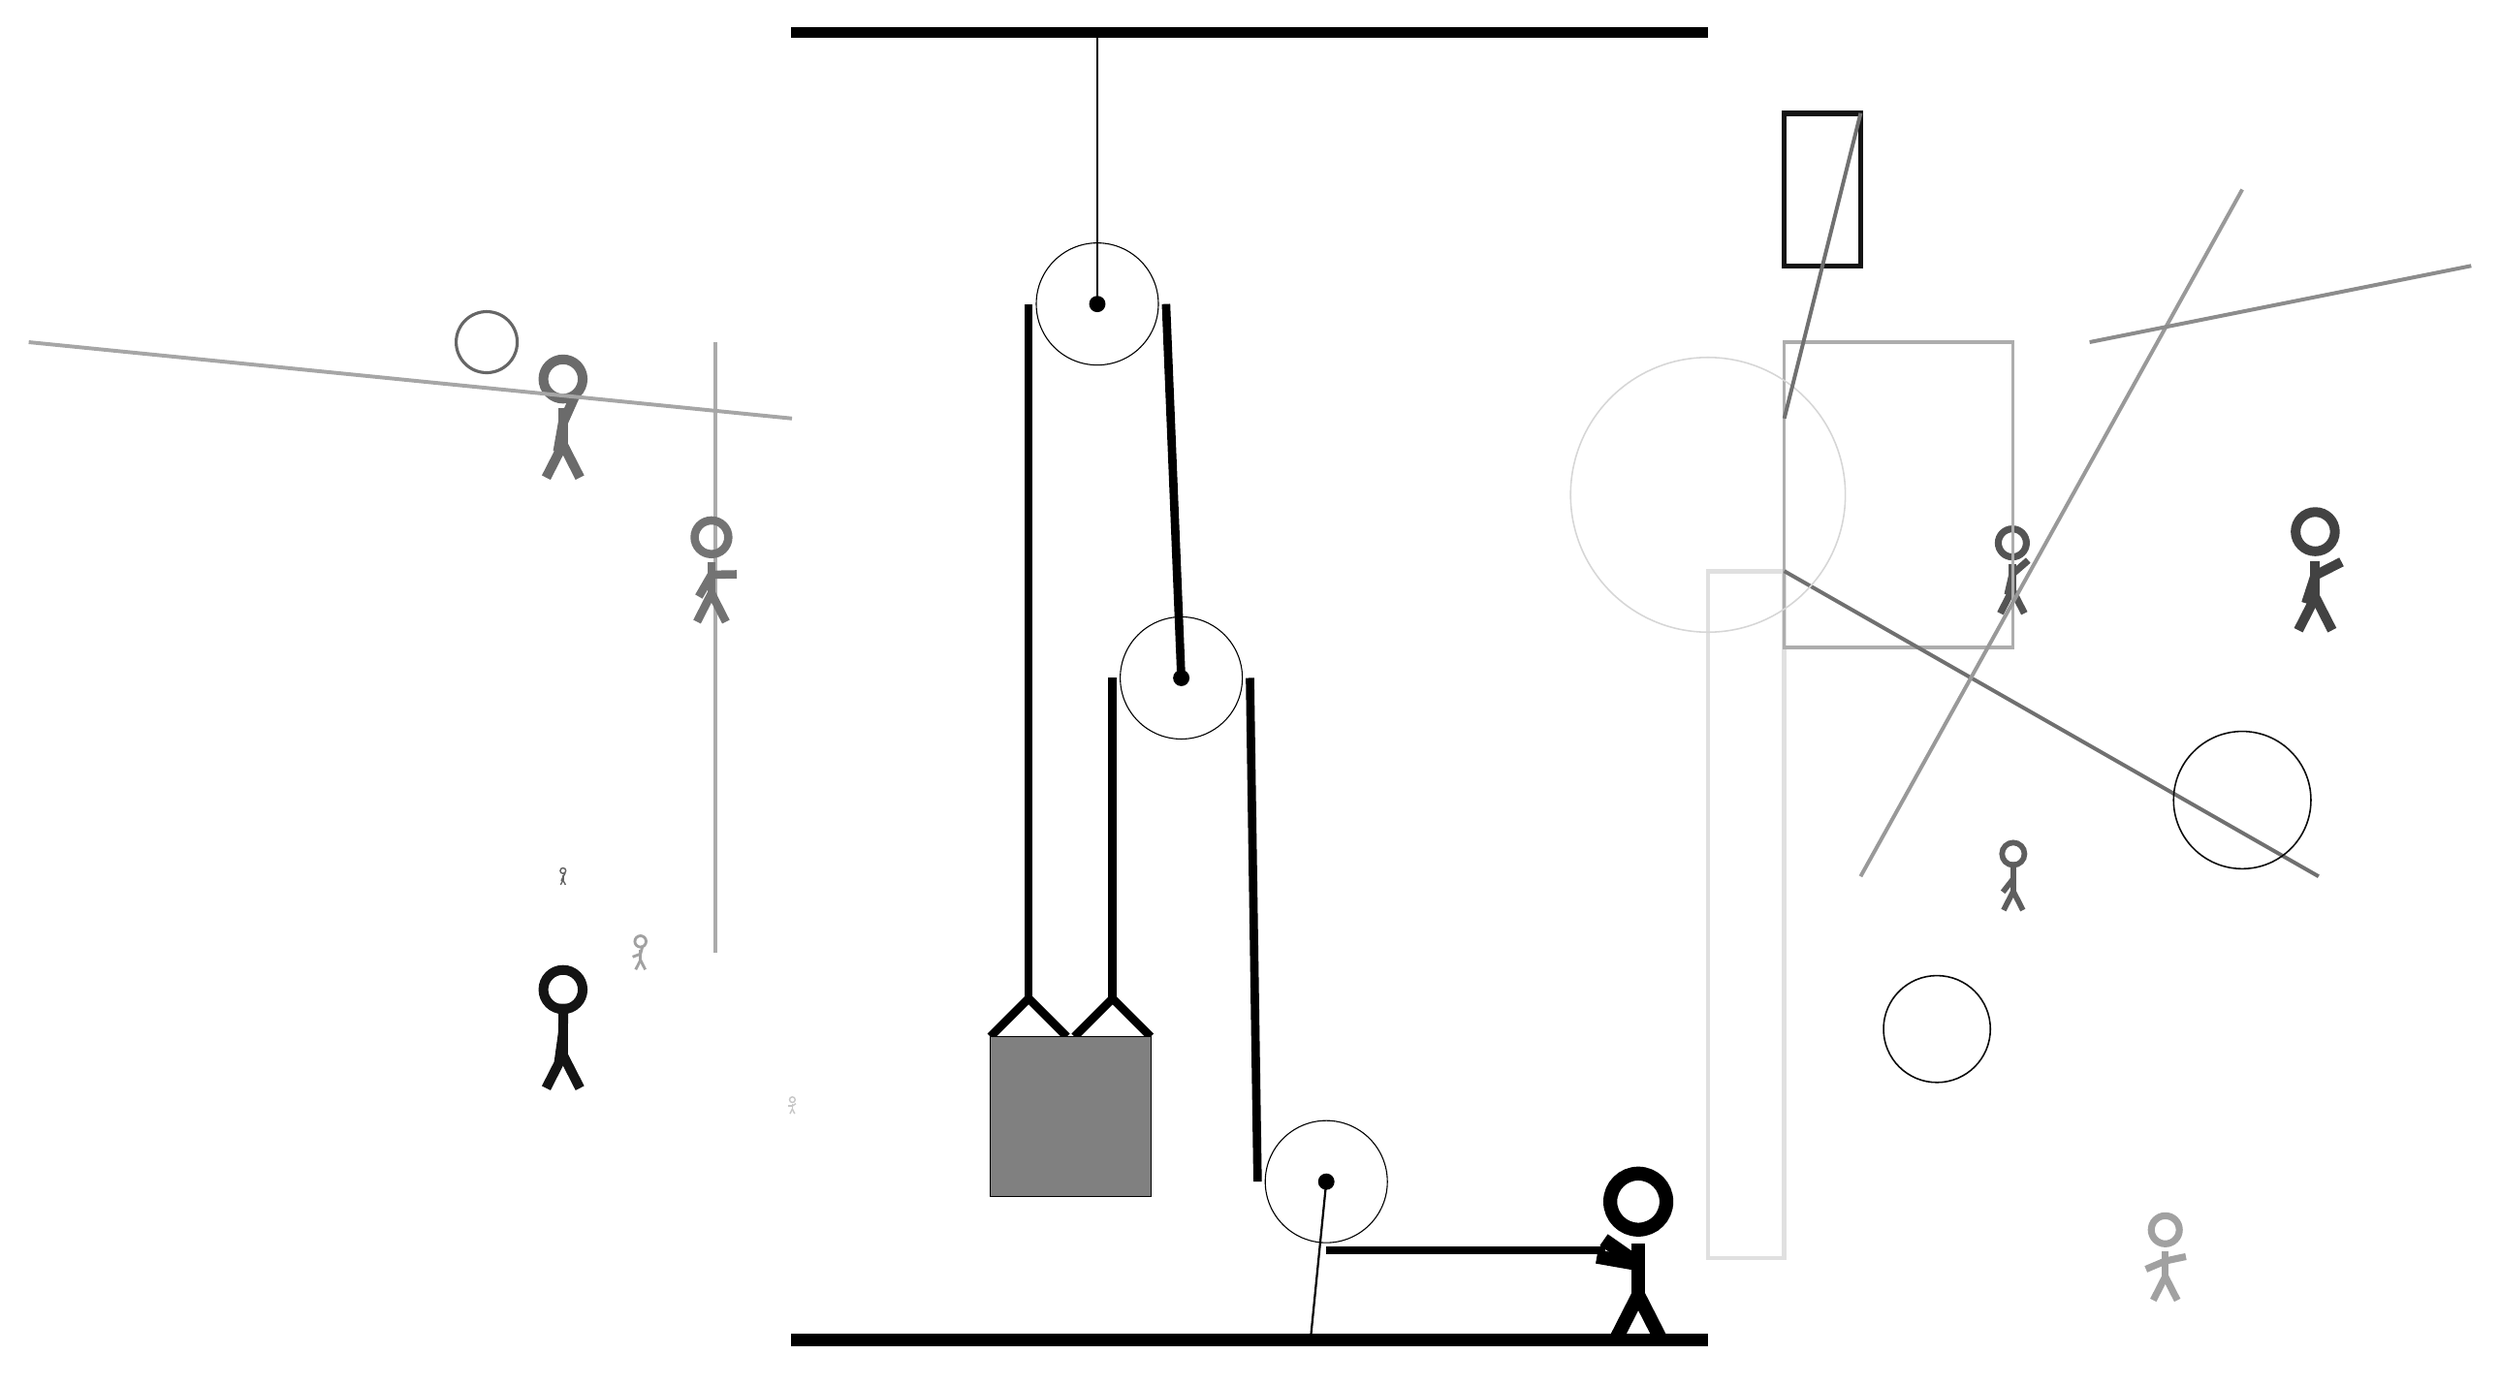
\begin{tikzpicture}
			%%%%% START %%%%%
			
			\draw[fill=black] (-2, 14) rectangle (10, 14.125);
			
			\draw (2, 10.5) circle (0.8);
			\draw[fill=black] (2, 10.5) circle (0.1);
			\draw[thick] (2, 10.5) -- (2, 14);
			
			\node[line width=0.7mm, color=black!58] at (-5, 9) {\Strichmaxerl[7][80][66]};
			
			\node[line width=0.2mm, color=black!67] at (14, 7) {\Strichmaxerl[5][77][41]};
			\draw [line width=0.4mm, color=black!60](-6, 10) circle (0.4);
			\node[line width=0.2mm, color=black!22] at (-2, 0) {\Strichmaxerl[1][0][33]};
			\node[line width=0.7mm, color=black!92] at (-5, 1) {\Strichmaxerl[7][82][89]};
			\draw[line width=0.6mm, color=black!12] (11, 7) rectangle (10, -2);
			\draw[line width=0.5mm, color=black!33] (-3, 2) rectangle (-3, 10);
			
			\node[line width=0.3mm, color=black!37] at (-4, 2) {\Strichmaxerl[2][21][75]};
			\node[line width=0.3mm, color=black!63] at (14, 3) {\Strichmaxerl[4][52][89]};
			\node[line width=0.5mm, color=black!74] at (18, 7) {\Strichmaxerl[7][72][27]};
			\draw [line width=0.4mm, color=black!39](-4, 9) circle (0.0);
			\draw[line width=0.4mm, color=black!32] (11, 6) rectangle (14, 10);
			\draw [line width=0.2mm, color=black!97](13, 1) circle (0.7);
			
			\draw[line width=0.5mm, color=black!56](11, 7) -- (18, 3);
			\draw [line width=0.2mm, color=black!16](10, 8) circle (1.8);
			\draw[line width=0.5mm, color=black!35](-2, 9) -- (-12, 10);
			\draw[line width=0.7mm, color=black!92] (12, 11) rectangle (11, 13);
			\draw[line width=0.5mm, color=black!40](12, 3) -- (17, 12);
			\node[line width=0.5mm, color=black!37] at (16, -2) {\Strichmaxerl[5][23][12]};
			\draw[line width=0.5mm, color=black!45](15, 10) -- (20, 11);
			\node[line width=0.3mm, color=black!61] at (-5, 3) {\Strichmaxerl[1][66][61]};
			
			\node[line width=0.7mm, color=black!55] at (-3, 7) {\Strichmaxerl[6][60][1]};
			\draw [line width=0.2mm, color=black!96](17, 4) circle (0.9);
			\draw[line width=0.5mm, color=black!56](12, 13) -- (11, 9);
			
			\draw (3.1, 5.6) circle (0.8);
			\draw[fill=black] (3.1, 5.6) circle (0.1);
			
			\draw (5, -1) circle (0.8);
			\draw[fill=black] (5, -1) circle (0.1);
			\draw[thick] (5, -1) -- (4.8, -3);
			
			\draw[line width = 1.1mm]  (0.6, 0.9) -- (1.1, 1.4) -- (1.6, 0.9);
			\draw[line width = 1.1mm]  (1.7, 0.9) -- (2.2, 1.4) -- (2.7, 0.9);
			\draw[fill=black!50] (0.6, 0.9) rectangle (2.7, -1.2);
			
			\draw[line width = 1.1mm] (1.1, 10.5) -- (1.1, 1.4);
			\centerarc[line width = 1.1mm](2, 10.5)(0:180:0.9);
			\draw[line width = 1.1mm] (2.9, 10.5) -- (3.1, 5.6);
			\draw[line width = 1.1mm] (2.2, 5.6) -- (2.2, 1.4);
			\centerarc[line width = 1.1mm](3.1, 5.6)(0:180:0.9);
			\draw[line width = 1.1mm] (4.0, 5.6) -- (4.1, -1);
			\centerarc[line width = 1.1mm](5, -1)(180:270:0.9);
			\draw[line width = 1.1mm] (5, -1.9) -- (8.65, -1.9);
			
			\node at (9, -2) {\Strichmaxerl[10][-35][170]};
			
			\draw[fill=black] (-2, -3) rectangle (10, -3.15);
			
			%%%%% END %%%%%
		\end{tikzpicture}
	\end{figure}	
\end{document}